\documentclass{ctexart}
\CTEXsetup[format={\Large\bfseries}]{section}
\newcommand{\jn}{JN}
\usepackage{graphicx}
\usepackage{float}
\usepackage{listings}
\begin{document}

\title{学习笔记--istio}
\author{mayidudu 来自 \jn}
\maketitle
%https://blog.csdn.net/wcx1293296315/article/details/79775671, 插图
\tableofcontents


\begin{center}
	本篇笔记用于记录istio学习过程中遇到的问题
\end{center}
\section{ServiceMesh}
“Service Mesh”概念还非常年轻,这个词在国内被翻译为“服务网格”或“服务啮合层”,我们这里就用Service Mesh这个英文词。这里摘录一下ServiceMesh中文社区上的一篇名为《年度盘点2017之Service Mesh:群雄逐鹿烽烟起[1]》的文章中对Service Mesh概念的回顾:在 2016 年年初,“Service Mesh”还只是 Buoyant 公司的内部词汇,而之后,它开始逐步走向社区:2016 年 9 月 29 日在 SF Microservices 上,“Service Mesh”这个词汇第一次在公开场合被使用。这标志着“Service Mesh”这个词,从 Buoyant 公司走向社区。2016 年 10 月,Alex Leong 开始在 Buoyant 公司的官方 Blog 中连载系列文章“A Service Mesh for Kubernetes”。随着“The Services must Mesh”口号的喊出,Buoyant 和 Linkerd 开始 Service Mesh 概念的布道。2017 年 4 月 25 日,William Morgan 发布博文“What’s a Service Mesh? And why do I need one?”。正式给 Service Mesh 做了一个权威定义。而Service Mesh真正引起大家关注要源于istio项目的开源发布。该项目由Google、IBM共同合作创建,Lyft公司贡献了Envoy项目将作为Istio Service Mesh的data panel。Google、IBM的影响力让Service Mesh概念迅速传播,同时也让大家认识到了Istio项目在Service Mesh领域的重要性,于是纷纷选择积极支持并将自己的产品或项目与Istio项目集成。

Service Mesh 提供了一种透明的、与编程语言无关的方式,使网络配置、安全配置以及遥测等操作能够灵活而简便地实现自动化。从本质上说,它解耦了服务的开发与运维工作。如果你是一名开发者,那么在部署新服务,或是修改现有服务的时候,就无需担心这些操作会对你的分布式系统带来哪些运维层面的影响。与之类似,运维人员可以放心地对服务之间的运维控制进行变更,而无需重新部署服务或是修改服务的源代码。处于服务与底层网络之间的这一层基础设施通常被称为 Service Mesh。


Google 内部通过一个分布式平台对服务进行管理,通过代理处理内部与外部的协议。这些代理的背后是一个控制面板,它在开发者与运维人员之间提供了一层额外的抽象,在这层抽象之上对跨语言与系统平台的服务进行管理。经过实战的检验,这套架构已经证明它能够确保高伸缩性、低延迟性,并为 Google 的各项服务提供了丰富的特性。

在 2016 年决定开发一个对微服务进行管理的开源项目,它与我们在 Google 内部使用的平台有很大的相似性。我们决定将该项目命名为“Istio”。之所以会取这样一个名字,是因为 Istio 在希腊语中的意思是“启航”。而在方案启动时就决定它需要支持 Kubernetes,而后者在希腊语中可以翻译为“舵手”或“驾驶员”。需要强调的是,Istio 对于服务部署环境并没有加以限定,它的开发目标就是能够管理在不同环境中运行的服务。

就在开始 Istio 项目开发工作的几乎同一时间,IBM 也发布了一个名为 Amalgam8 的开源项目,这是一个基于 NGINX 技术,为微服务提供基于内容的路由方案的项目。随后,IBM 意识到这两个项目在使用场景与产品愿景上存在很大一部分交集,于是答应成为合作伙伴,放弃 Amalgam8 的开发,共同基于 Lyft公司 的 Envoy 项目打造 Istio 这款产品。

Istio项目是Service Mesh概念的最新实现,旨在所有主流集群管理平台上提供Service Mesh层,初期以实现Kubernetes上的服务治理层为目标。

\section{istio是什么}
一个用来连接、管理和保护微服务的开放平台。 
Istio提供一种简单的方式来建立已部署服务网络,具备负载均衡、服务间认证、监控等功能,而不需要改动任何服务代码。
想要为服务增加对Istio的支持,您只需要在环境中部署一个sidecar,使用Istio控制面板功能配置和管理代理,拦截微服务之间的所有网络通信。


\section{istio的架构}
\begin{figure}[H]
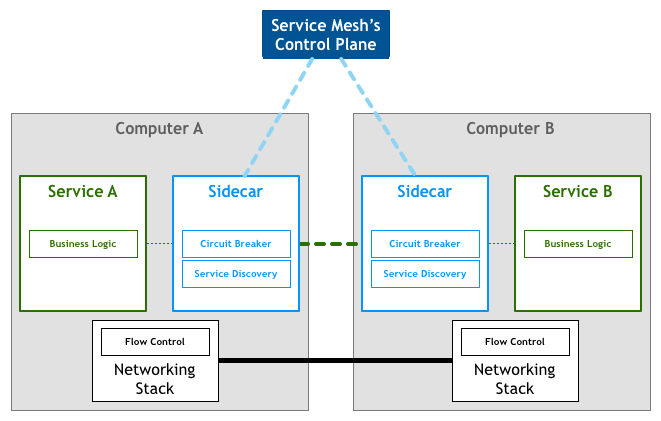
\includegraphics[scale=0.6]{istio/framework.png}
\caption{istio架构}
\end{figure}

\begin{figure}[H]
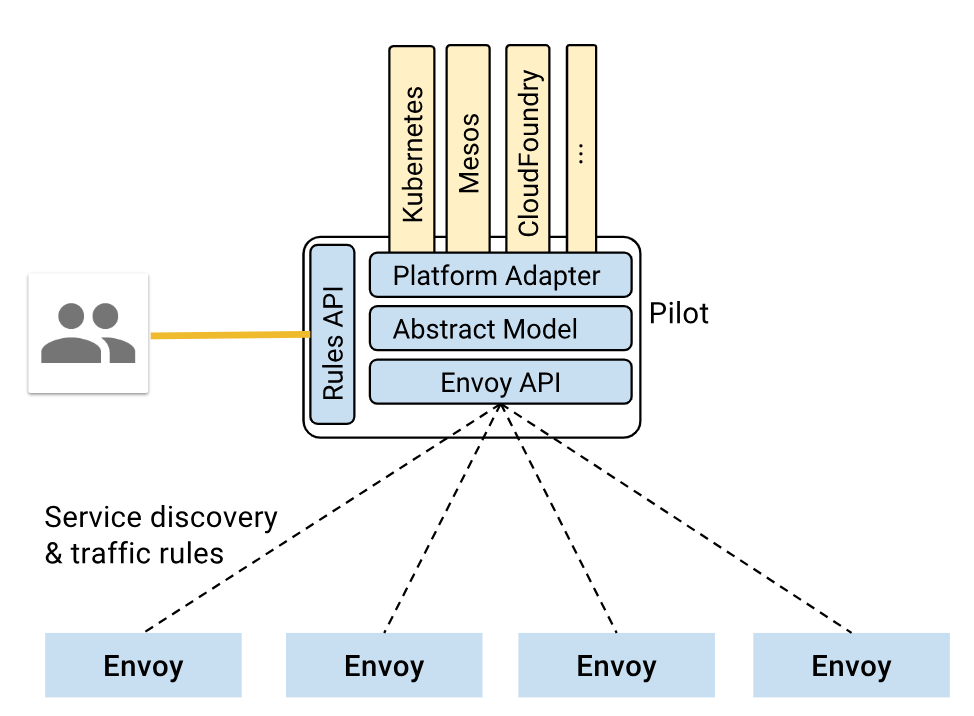
\includegraphics[scale=0.4]{istio/istion_component.png}
\caption{组件}
\end{figure}


分为控制平面和数据平面两部分。 
\begin{enumerate}
	\item [-] 控制平面:Pilot, Mixer, Istio-Auth,分别对Istio中的服务做流量管理,策略配置,安全通信等规则配置 
	\item [-] 数据平面:所有pod上的Envoy,负责所有规则的执行
\end{enumerate}
\begin{figure}[H]
	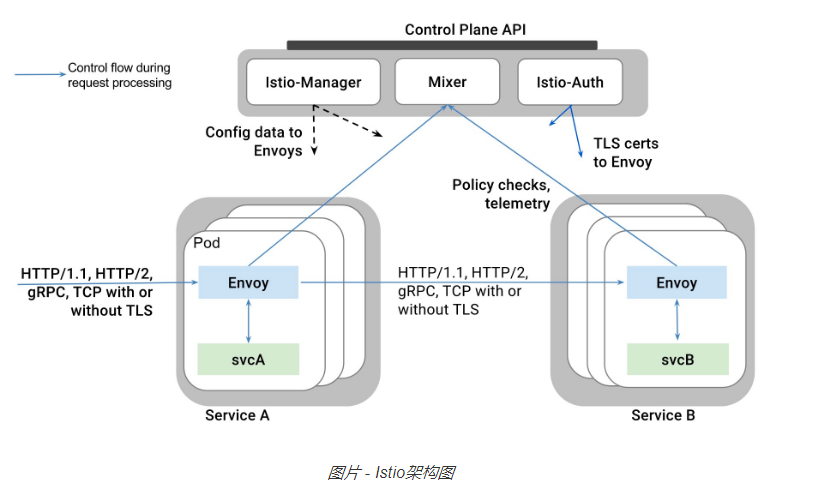
\includegraphics[scale=0.5]{istio/framework2.png}
	\caption{istio分层结构}
\end{figure}
Sidecar中Envoy代理了Pod中真正业务Container的所有进出流量,并对这些流量按照控制平面设定的“治理逻辑”进行处理。而这一切对Pod中的业务应用是透明的,开发人员可以专心于业务逻辑,而无需再关心微服务治理的逻辑。Istio代表的Service Mesh的设计理念被认为是下一代“微服务统一框架”,甚至有人认为是微服务框架演化的终点。
Istio于2017年5月24日发布了0.1 release版本,目前已经到release1.1,并且已经部署在云平台,如华为云。
代理

Envoy 是由 Lyft 公司基于 C++ 编写的一个高性能、开源的分布式代理(在 Lyft 公司内部用于处理生产环境中的网络请求)。Envoy 作为 sidecar 部署在系统中,对所有流入与流出的网络请求进行拦截,实现各种网络策略,并与 Istio 控制面板集成。Istio 利用了 Envoy 内建的大量特性,例如服务发现与负载均衡、流量拆分、故障注入(fault injection)、熔断器以及分阶段发布等功能。

Pilot

作为控制面板的重要组成部分之一,Pilot 负责管理代理的配置,并将服务的通信策略分发至 Istio mesh 中所有的 Envoy 实例。它能够接受高级别的规则(例如发布策略),将其解释为低级别的 Envoy 配置,并将配置分发至 sidecar,而且不会导致停机或是重新部署。虽然 Pilot 本身不依赖于底层平台,但运维人员可以利用特定于平台的适配器,将服务发现的信息推送给 Pilot。

Mixer

Mixer 能够在 Istio 中集成各种生态的基础设施后端系统,它通过即插即用的适配器集,通过标准的配置模型,使 Istio 能够方便地与现有的服务进行集成。适配器对 Mixer 的功能进行了扩展,并将特定的接口暴露给监控、日志、追踪、配额管理及其他功能。适配器是按需加载的,并按照运维人员的配置在运行时发挥作用。

Citadel

Citadel 即之前的 Istio Auth,它为跨 mesh 的服务与服务之间的通信进行证书签名与轮换,提供双向认证与双向授权功能。Envoy 通过 Citadel 证书,在每个调用中以透明的方式注入双向的TLS,通过自动化的身份与凭证管理,对流量进行安全管理与加密。Citadel 符合 Istio 的整体设计,只需少量的服务代码(甚至完全不需要服务代码)即可配置认证与授权功能,并且能够无缝地支持多个集群与平台。


\section{istio的主要功能}
流量管理(Pilot)。控制服务之间的流量和API调用的流向,使得调用更灵活可靠,并使网络在恶劣情况下更加健壮。

可观察性。通过集成zipkin等服务,快速了解服务之间的依赖关系,以及它们之间流量的本质和流向,从而提供快速识别问题的能力。

策略执行(mixer)。将组织策略应用于服务之间的互动,确保访问策略得以执行,资源在消费者之间良好分配。策略的更改是通过配置网格而不是修改应用程序代码。

服务身份和安全(Istio-auth)。为网格中的服务提供可验证身份,并提供保护服务流量的能力,使其可以在不同可信度的网络上流转。

除此之外,Istio针对可扩展性进行了设计,以满足不同的部署需要:

平台支持。Istio旨在可以在各种环境中运行,包括跨云、预置环境、Kubernetes、Mesos等。最初专注于Kubernetes,但很快将支持其他环境。
集成和定制。策略执行组件可以扩展和定制,以便与现有的ACL、日志、监控、配额、审核等解决方案集成。

\section{istio的优势}
Istio 具有高度模块化的特性,适用于多种场景。对于它带来的各种益处的详细解释可能已经超出了本文的范围,但我还是会简单地做个介绍,体验一下如何通过它简化网络运维、安全运维以及 DevOps 的日常工作。

\textbf{灵活性}

Istio 能够保护应用不被片状网络和雪崩式故障所影响。如果你是一位网络 运维人员,就可以通过故障注入等特性在系统中注入网络延迟及网络隔离等故障,系统性地检验应用的灵活性。如果你希望将某个版本的服务迁移至另一个版本,可通过基于权重的流量路由方式,逐渐将流量导向新版本的服务,以此降低风险。更好的办法是,在进行实际的切换之前,你可以模拟出真实的流量指向新的部署服务的行为,以观察它的运行情况。此外,你还可以通过 Istio Gateway 对流入与流出的流量进行负载均衡,并对流量应用各种路由规则,例如超时、重试以及熔断等等,以减少潜在的故障,并从故障中恢复。

\textbf{安全性}

Istio 的一个主要使用场景是在异构的系统中对服务间的通信进行安全加密。安全运维人员能够以统一的方式进行大规模的操作,例如开启流量加密、在不破坏其他服务的前提下阻止对某个服务的访问、开启双向身份认证、通过访问控制(ACL)管理服务白名单、对服务与服务间的通信进行授权,以及分析服务的安全性状况等等。运维人员可以在单个服务、单个命名空间或整个 mesh 的范围内实施这些安全策略。这些功能的存在可以减少对于防火墙层次的依赖,减少安全运维人员的工作负担。

\textbf{可观测性}

微服务所带来的一大挑战是如何以可视化方式了解基础设施的运行情况。直至近期,最佳的方式仍然是对每个服务进行扩展,以实现端到端的服务交付。除非你打算投入一个团队的人力专门对二进制文件进行调整,否则仍然很难对整个平台有一个全局性的认识,对于系统瓶颈的故障诊断依然十分不便。

而通过 Istio 自带的功能,你就可以通过可视化的方式了解系统的关键指标,并且能够跨服务进行请求的追踪。如此一来,你就可以实现基于应用指标进行自动扩展等操作。虽然 Istio 支持多种扩展,例如 Prometheus、 Stackdriver、Zipkin 和 Jaeger 等等,但其本身并不受限于后端平台的选择。如果你找不到趁手的工具,完全可以自行编写适配工具,与 Istio 进行集成。








\section{基本概念}

\subsection{Traffic Management}
	使用 istio 的流量管理模型实质上解耦了 traffic flow 和 infrastructure scaling,
你可以通过 Pilot 指定 traffic 遵循的规则, 然后由 Pilot 和 Envoy 来做其余的事情,  而不是直接指定让哪个 Pods/VMs 接收 traffic.
\begin{enumerate}
	\item [*] \textbf{Pilot and Envoy:}
在 istio 中用于 traffic management 的核心组件就是 Pilot, 它管理和配置部署在 service mesh 中的 envoy.
Pilot 让你指定你想使用哪些规则来路由Envoy proxies 之间的 traffic , 并配置 failure recovery 特性,例如 timeouts, retries, circuit breakers.
它还维护一个网格中所有服务的 canonical model (规范模型) , 并且使用这个模型 让envoy实例 通过它的 discovery service 知道网格中的其他envoy实例的存在.
每个 envoy 实例都维护一份 load balancing 信息, 这份信息基于它从 Pilot 获取的信息, 并且周期性地对位于其 load-balancing pool 中的其他实例进行健康检查, 从而允许它可以在遵循指定的路由规则的同时也能智能地在目标实例之间分配流量.
Pilot 负责部署在服务网格中的 envoy实例 的生命周期.

	
	\item [*] \textbf{Request routing:}
	在istio中一个服务的模型和其在底层平台(例如kubernetes,Mesos,Cloud foundry(代工厂)等等)的表示形式无关.
	Platform-specific adapters 负责将 istio中的服务模型 polulating 到指定平台.
	istio 引进了 服务版本 的概念, 这可以区分不同版本的服务或不同环境的服务, 而且一般多哟用于 A/B测试 和 金丝雀发布.
	对于服务调用方而言, 它们不知道服务版本的存在. 它们面对的还是原来的服务,没有变化.  envoy 负责解析并转发 client 和 service 直接的请求和响应.
	envoy 可以根据你通过 Pilot 制定的路由规则 选择服务, 可以根据请求的 headers, 源/目的地的tags, 或者某个版本的weight 来进行路由.
	istio 不提供DNS, 应用可以尝试使用底层平台提供的DNS服务(例如 kube-dns, mesos-dns 等等)
	
	\item [*] \textbf{Ingress and egress:}
	istio 假设所有的进入和离开服务网格的流量 都是通过 envoy 代理的.
	istio 假设已经存在一个服务注册表用于追踪服务的 pods/VMs . istio 还假设一个服务的新实例会自动注册到服务注册表中, 并且不健康的实例会自动移除.  底层平台(例如kubernetes和Mesos)已经为基于容器的应用提供了这些功能, 并且基于VM的应用也有很多已经存在的解决方案.
	Pilot 消费服务注册表中的服务信息, 并提供一个平台无关的 服务发现接口.  服务网格中的envoy实例就从这个接口获取信息.
	
	\item [*] \textbf{handling failures:}
	envoy 提供了一套 out-of-the-box(开箱即用)的选项用于故障恢复功能,  这些功能包括:
	
	超时返回: Timeouts\\
	重试: Bounded retries with timeout budgets and variable jitter between retries\\
	到upstream服务的并发连接数和请求数限制: Limits on number of concurrent connections and requests to upstream services\\
	对负载均衡池中的服务的周期性的主动健康检查: Active (periodic) health checks on each member of the load balancing pool\\
	细粒度的断路器(被动的健康检查): Fine-grained circuit breakers (passive health checks) – applied per instance in the load balancing pool
	
	这些功能可以在 运行时 动态配置, 通过 istio 的 traffic management 的 rules.
	
	\item [*] \textbf{Fine tuning:}
	Istio’s traffic management rules 允许你设置每个服务的默认的 failure discovery, 和默认的服务版本.
	然而, 服务的消费者也可以通过特定的HTTP请求头 来覆盖默认的 timeout 和 重试次数, 在 envoy 作为proxy时,这些头是 x-envoy-upstream-rq-timeout-ms and x-envoy-max-retries .
	
	\item [*] \textbf{Fault injection}

	既然 envoy 提供了 服务的 failure recovery 机制, 那么同时使用 envoy 来进行 end-to-end 的 failure recovery capability 也势在必行.
	错误配置的 failure recovery policies 会引起持续的关键服务的不可用, 这会导致可怜的用户体验.
	istio 能够进行 protocol-specific fault injection into the network, 而不用 杀掉 pods 或 延迟或破坏 TCP层的包.  这样做的理由是, 无论网络级故障如何,应用层观察到的故障都是相同的,并且可以在应用层注入更有意义的故障(例如,HTTP错误代码)以实现应用程序的弹性。
	


\end{enumerate}

\subsection{Rule configuration}
istio 提供了一个简单的配置模型 用于控制在不同服务之间的 API调用和layer-4 traffic flow.
这个配置模型允许你配置 服务级别的 属性,例如 ircuit breakers, timeouts, and retries, 还能配置持续的发布,例如 canary rollouts, A/B testing, staged rollouts with %-based traffic splits 等等.
在 istio 中有 4 个关于 traffic management 的配置资源:

VirtualService: VirtualService 定义了 在服务网格内 对一个 istio服务 的请求应该如何被路由. 例如到某个 destination rule 或 某个k8s中的服务.

DestinationRule: DestinationRule 配置不同版本的服务.

ServiceEntry: ServiceEntry 一般用于让应用可以访问istio服务网格之外的服务.

Gateway: Gateway 为 HTTP/TCP traffic 配置一个 load balancer , 一般工作于网格边缘,作为整个应用的入口

\begin{enumerate}
	\item [*] \textbf{virtualService}
	
	下面的 VirtualService 定义了 将访问 istio中的reviews 服务的100%流量都路由到 k8s中的 reviews 服务的v1版本
\lstset{language=C}
\begin{lstlisting}
apiVersion: networking.istio.io/v1alpha3
kind: VirtualService
metadata:
  name: reviews
spec:
  hosts:
  - reviews
  http:
  - route:
    - destination:
      host: reviews
      subset: v1


\end{lstlisting}

	VirtualService 可以基于 请求的 source 和 destination, HTTP paths 和 header fields, 服务的不同版本的权重等信息对请求进行路由.
	Routing rules(路由规则) 对应于 在 VirtualService 的配置中指定的一个或多个 destination hosts . 这些 hosts 可能和实际的 destination 负载相同,也可能不同, 甚至可能是网格中不可路由的服务.
	例如, 要定义 请求 reviews 的服务, 可以通过其内部的网格服务名称 review 或 通过主机 bookinfo.com , VirtualService 可以这样定义它的 hosts field :
	

	
\end{enumerate}

\subsection{Polices and Telemetry}
Istio 提供了一种灵活的模型 来实施 authorization policies 和 收集网格中服务的 telemetry .
底层架构负责提供用于构建服务的功能.  这些功能包括 访问控制系统, telemetry 收集系统, 配额实施系统, 计费系统等等. 传统上, 服务直接与底层架构集成, 这构成了 硬耦合和 baking-in specific semantic 和 usage options.
istio 提供了一个统一的抽象模型, 这使得 istio 可以与一组开放式的底层架构交互.
这样做是为了向运营商提供丰富和深入的控制,同时不给服务开发者带来负担.
istio 旨在改变层之间的界限, 以降低系统复杂性, 从 service 代码中消除 policy logic 并给予用户控制权.
Mixer 是 istio 组件, 它负责提供 policy controls 和 收集 telemetry .
Envoy sidecar 在每次请求之前先调用 Mixer 执行前置条件检查, 并在请求之后报告 telemetry.
sidecar 会在本地缓存这些检查策略, 因此可以使用缓存执行大部分前置检查条件.
另外, sidecar 也会缓冲 outgoing telemetry, 使得它不用那么频繁的调用 Mixer.
At a level , Mixer 提供了:

Backend Abstraction: 后端抽象, Mixer 将 istio的其他部分与底层架构的实现细节 隔离开来.
Intermediation: 中介, Mixer 允许操作者对 网格和底层架构 之间的交互进行 细粒度的控制.

除了这些功能之外, Mixer 还具有如下所述的可靠性和可扩展性优势:
Policy 实施和telemetry 收集完全由配置来驱动, 你可以完全禁用这些特色并避免在部署istio时运行 Mixer 组件.
\begin{enumerate}
	\item [+] 1. Adapters
	Mixer 是一个高度 模块化和可扩展的组件.
	其关键功能之一就是抽象出 不同policy和telemetry 后端系统的细节, 允许 istio 的其他部分与这些后端无关.
	Mixer 的这种可以处理不同底层架构后端的灵活性来自于它的 通用插件模型.
	插件就是 Adapters, 它们允许 Mixer 连接到不同的底层架构后端提供核心功能, 例如 logging, monitoring, quotas, ACL checking 等等.
	使用哪些Adapter是在运行时配置的, 并且可以轻松地扩展到新的目标或自定义的后端架构.
	\item [+] 2. 可靠性和延迟
	Mixer 是一个高可用的组件 :
	\begin{enumerate}
		\item [$\bullet$] Statelessness 无状态: Mixer 是无状态的, 所以它不会管理任何的持续性存储.
		\item [$\bullet$] Hardening : 强壮: Mixer 的目标是被设计为一个高可靠的组件. 每个单独的 Mixer 实例提供 99.999% 的 uptime
		\item [$\bullet$] Caching and Buffering:
		
	\end{enumerate}
\end{enumerate}






\section{应用领域}

\section{研究重点}



\begin{table}[h]
	\centering
	\caption{研究步骤}
	\begin{tabular}{|c|c|}
		\hline
		顺序 & 步骤 \\\hline
		1 & \textbf{安装测试基本功能} \\\hline
		2 & \textbf{阅读源码} \\\hline
		3 & \textbf{能够进行编译} \\\hline
		4 & \textbf{了解基础架构并能够进行修改} \\\hline
	\end{tabular}
\end{table}

\begin{table}[h]
	\centering
	\caption{研究时间安排}
	\begin{tabular}{|c|c|}
		\hline
		2018-12-31 & 测试环境构建 \\\hline
		2019-01-15 & 了解基本的源码架构 \\\hline
	\end{tabular}
\end{table}

\section{istio测试环境}
\subsection{基础资源需求}

\begin{table}[h]
	\centering
	\caption{测试环境}\label{tab:tab1}
	\begin{tabular}{|c|c|c|}
		\hline
		服务器 & 2个vm & fusion \\\hline
		OS & Centos7 & 固定硬盘 \\\hline
		Mem & 4G  & 支持Docker部署 \\
		\hline
	\end{tabular}
\end{table}


\subsection{部署结构}


\section{istio与spring cloud比较}
istio是无侵入式的,可以支持多语言,而spring cloud是针对java平台的。

\section{问题}
\subsection{Istio的发展现状如何?}

新的特性正在不断地加入 Istio 中,同时,我们也在改进现有的功能。Istio 的开发遵循标准的敏捷风格,每个特性都需要通过自身的生命周期进行交付(dev/alpha/beta/stable)。虽然有一部分功能仍在改进中,但有许多功能已经可以在生产环境中使用了(beta/stable)。欢迎在 istio.io 网站上查看最新的功能列表。

Istio 遵循严格的发布节奏,虽然我们提供每日和每周构建的版本,但并不提供相应的支持,也不确保其可靠性。另一方面,每月构建的 snapshot 版本则相对更安全,并且通常会包含新的特性。不过,如果你打算在生产环境中使用 Istio,请选择包含“LTS”(长期支持)标签的版本。在本文编写时,最新的 LTS 版本号是 0.8。你可以在 GitHub 上找到该版本以及其他各版本。

\subsection{后续有什么计划?}

自从在 GlueCon 大会上正式发布 Istio 0.1 版本以来,已经过了一年时间。虽然我们取得了很大的进展,但仍有许多工作需要完成。近期的目标是在关键的功能都进入 beta 阶段(某些情况下或许需要等待 stable 阶段)后发布 Istio 1.0 版本。需要指出的是,该版本并非 Istio 功能的全部,而只是我们基于社区的反馈,所选出的最重要功能。为了本次发布,我们也在尽力改进一些非功能性的需求,例如性能与扩展性,同时也在改进我们的文档以及上手体验。

Istio 的一个重要目标是支持混合型环境。举例来说,用户可以将虚拟机运行在 GCE、本地 Cloud Foundry 集群,或是其他公有云的服务上。Istio 能够为整体服务平台提供一个统一的视图,管理这些环境之间的连接并确保安全性。我们目前正在致力于实现多集群的架构,允许你在扁平网络中将多个 Kubernetes 集群加入一个单独的 mesh 中,并启用跨集群的服务发现功能,这项工作在 0.8 LTS 版本中还处于 alpha 阶段。在不远的将来,它还将支持全球化的集群级别的负载均衡,并通过 Gateway 对等互联提供对非扁平网络的支持。

除了 1.0 版本的发布之外,另一个工作重心是 API 管理功能。计划推出一个 service broker API,它能够对各个服务提供服务发现与上线功能,将服务消费者与服务管理者相关联在一起。我们还将为 API 管理功能提供一个统一的接口,这些功能包括 API 业务分析、API 密钥验证、认证检验(例如JWT、OAuth等等)、编码转换(JSON/REST 至 gRPC 转换)、路由,以及与多种 API 管理系统的集成,例如 Google Endpoints 与 Apigee。

所有这些短期目标都是为了最终实现长期目标,即将 Istio 融入至不同的环境中。按照技术主管同时也 Istio 的创始者 Sven Mawson 所说:“我们所希望实现的理想,是让 Istio 能够融入每个环境中,无论你使用的是哪一种环境或平台,都能够为你提供服务管理的功能“。

虽然 Istio 仍然处于早期阶段,但它的开发速度与接受度正在稳步地提升。无论对于主流云厂商还是个人贡献者来说,Istio 都已经成为了 Service Mesh 的代名词,同时也是基础设计发展路线图中的一个重要组成部分。每一次的发布,都意味着我们向目标更近了一步。
\subsection{istio 服务无法访问外网问题}
缺省情况下,启用了Istio的服务是无法访问外部URL的,这是因为Pod中的iptables把所有外发传输都转向到了Sidecar代理,而这一代理只处理集群内的访问目标。

我们可在Istio集群中使用两种方式来访问外部服务:
使用Egress规则。
配置Istio Sidecar,在他的iptables中排除对外部IP的控制。 
Egress 规则
配置Istio Sidecar 
让指定IP范围直接穿透Istio,就需对源服务的Envoy Sidecar进行配置,阻止其对外部请求的拦截。

通过--includeIPRanges指定。

% kubectl apply -f <(istioctl kube-inject -f samples/sleep/sleep.yaml --includeIPRanges=10.0.0.1/24)

%IPranges即service的IP范围,在kube-api_server.service中通过–service-cluster-ip-range指定。

\end{document}